\section{Historical controls with an extrapolation-first WSP prompt}\label{app:historical}
This preliminary study used an extrapolation-first prompt and included affine arithmetic and memoryless sum controls. All counts in this appendix refer to that earlier design. A network's \emph{architecture} specifies which operations it applies and where coefficients can enter. For the scalar tests, an \emph{affine} function multiplies input values by fixed coefficients, sums them and adds a constant. A \emph{rectified linear unit} (ReLU) is the scalar function $R(u)=\max(0,u)$ of a real input $u$. Let $w$ count the hidden units, let $a,b$ denote the slope and offset of a direct input-to-output path (a \emph{skip}), and give hidden unit $j$ input slope $u_j$, offset $v_j$ and output weight $c_j$. The shallow network computes
\[
                 f(x)=ax+b+\sum_{j=1}^{w}c_j R(u_jx+v_j).
\]
Each hidden unit contributes a \emph{hinge}, a possible change of slope at its zero crossing (a \emph{knot}). This architecture has $3w+2$ scalar slots.

We tested the square, sine in radians, positive self-power $x^x$, hyperbolic tangent $\tanh x=(e^{2x}-1)/(e^{2x}+1)$ with $e$ the base of the natural logarithm, addition, subtraction, running sum, sorting four inputs in ascending order, Fibonacci numbers, and triangular numbers. At integer index $n\ge0$, Fibonacci numbers start at $F_0=0,F_1=1$ and obey $F_{n+2}=F_{n+1}+F_n$. The triangular number is $T_n=n(n+1)/2$. Self-power uses positive real inputs. Appendix~\ref{app:signed} handles the separate negative-integer extension.

For each task and each of three random starts, two independent Astra requests saw the same three architectures, weights, deployment envelope and labeled examples. One request supplied \emph{the formula and examples}. The other supplied \emph{examples only}, omitting the task name and rule. Each request returned three complete arrays. This gives 60 calls and 180 WSP arrays. All 180 could be executed. The three arrays from a single call are dependent. This protocol allows a complete overwrite. Only Section~\ref{sec:front} minimizes edits. For each of the 90 task, size and start combinations we also fit all slots using BP with 800 Adam updates followed by up to 1,000 BFGS iterations. Each solver saw 12 central examples except on the integer-sequence tasks, which used indices 0 through 8. WSP was asked to prioritize the \emph{largest} scaled error. BP minimized half the \emph{mean squared} scaled error. Architectures, examples and initial arrays were paired. Objectives, prior knowledge and computational budgets differed.

\begin{table}[htbp]\centering\small\setlength{\tabcolsep}{3.5pt}
\caption{Held-out outer predictions on the same networks. Each method has an exact-match percentage and a raw root mean squared error (RMSE). Entries are medians over three starts. Formula and examples and examples only are the two weight-space programming (WSP) conditions. The backpropagation condition receives examples only. Scalar scores use 2,048 inputs per available shell side. Addition, subtraction, running sum and sorting each use 2,048 inputs or lists. A list must match at every position. Each Fibonacci or triangular score uses the 32 indices from 33 through 64 of one trajectory.}\label{tab:paired}
\begin{tabular}{@{}lr rr rr rr@{}}\toprule
&&\multicolumn{2}{c}{\textbf{WSP}}&\multicolumn{2}{c}{\textbf{WSP}}&\multicolumn{2}{c}{\textbf{Backpropagation}}\\
&&\multicolumn{2}{c}{Formula and examples}&\multicolumn{2}{c}{Examples only}&\multicolumn{2}{c}{Examples only}\\
\cmidrule(lr){3-4}\cmidrule(lr){5-6}\cmidrule(l){7-8}
Target & Slots & Exact \% & RMSE & Exact \% & RMSE & Exact \% & RMSE\\\midrule
$x^2$ & 50 & 0.0 & 0.644 & 0.0 & 0.633 & 0.0 & 29.5\\
$\sin x$ & 50 & 0.0 & 0.0335 & 0.0 & 0.0324 & 0.0 & 2.46\\
$x^x$, positive & 50 & 0.0 & $1.3\times 10^{8}$ & 0.0 & $1.3\times 10^{8}$ & 0.0 & $1.6\times 10^{9}$\\
$\tanh x$ & 50 & 0.0 & 0.00154 & 0.0 & 0.0015 & 0.0 & 0.52\\
Addition & 2 & 100.0 & 0 & 100.0 & 0 & 27.2 & $2.3\times 10^{-15}$\\
Subtraction & 2 & 100.0 & 0 & 100.0 & 0 & 1.3 & $4.7\times 10^{-15}$\\
Running sum & 3 & 100.0 & 0 & 100.0 & 0 & 0.0 & $2.3\times 10^{-14}$\\
Sort four & 40 & 53.5 & $5.2\times 10^{-16}$ & 53.6 & $5.0\times 10^{-16}$ & 0.6 & 5.95\\
Fibonacci & 8 & 100.0 & 0 & 100.0 & 0 & 0.0 & 0.269\\
Triangular & 15 & 100.0 & 0 & 100.0 & 0 & 0.0 & $2.1\times 10^{-8}$\\
\bottomrule
\end{tabular}
\end{table}

For this preliminary study, Table~\ref{tab:paired} uses the largest tested shallow scalar width (16 hinges) and the smallest tested size known to suffice over the reals for each algorithmic task. Both WSP conditions achieved perfect outer scores on addition, subtraction, running sum, Fibonacci and triangular numbers at those sizes. The examples-only condition still exposed a task-specific graph and recognizable labels. At width 16 all four smooth targets had zero exact outer matches for either WSP condition and for BP. On square, however, examples-only WSP had RMSE 0.633 versus 29.5 for BP. For sorting, formula-and-examples WSP matched only 53.5\% of complete vectors, but its RMSE was $5.2\times10^{-16}$. With a gradient fit the corresponding values were 0.6\% and 5.95. Appendix~\ref{app:additional} retains the scale-adjusted results, which reveal a different aspect of errors on rapidly growing $x^x$.

\paragraph{How close was each fit to the best training loss?}
The training loss is half the mean of $[(\hat y_i-y_i)/\max(1,|y_i|)]^2$ over observed scalar outputs. For the 12 one-hinge settings (four smooth functions and three starts), we computed the globally smallest \emph{real-arithmetic} loss on the stored binary64 labels by enumerating all intervals in which the knot can lie. For a second gradient-based optimizer, \emph{trust-region least squares} fits a local linear approximation of all output errors and restricts the update to a neighborhood where that approximation is useful. We applied it both at the original weights and after WSP.

Using an absolute training-loss gap of $10^{-10}$ to the certified optimum, Adam succeeded in 0/12 settings, Adam followed by BFGS in 1/12, and trust-region least squares from the same Xavier weights in 5/12. Starting least squares from examples-only WSP raised that to 9/12. Among the 90 settings, least squares from Xavier obtained six completely exact outer sets, all on addition or subtraction. In contrast, both WSP conditions obtained 30/90. The stronger optimizer improved a central objective without guaranteeing transfer. Refining the formula-and-examples WSP arrays reduced training loss materially in 54 settings. It improved outer mean scaled absolute error in seven and worsened it in 47. Figure~\ref{fig:optim} gives the paired counts. Appendix~\ref{app:optimizer} reports the per-task RMSE comparisons, solver budgets and optimality argument. Appendix~\ref{app:convex} repeats the comparison with hidden units frozen so that the output weights admit an exact least-squares characterization.

\begin{figure}[htbp]
\centering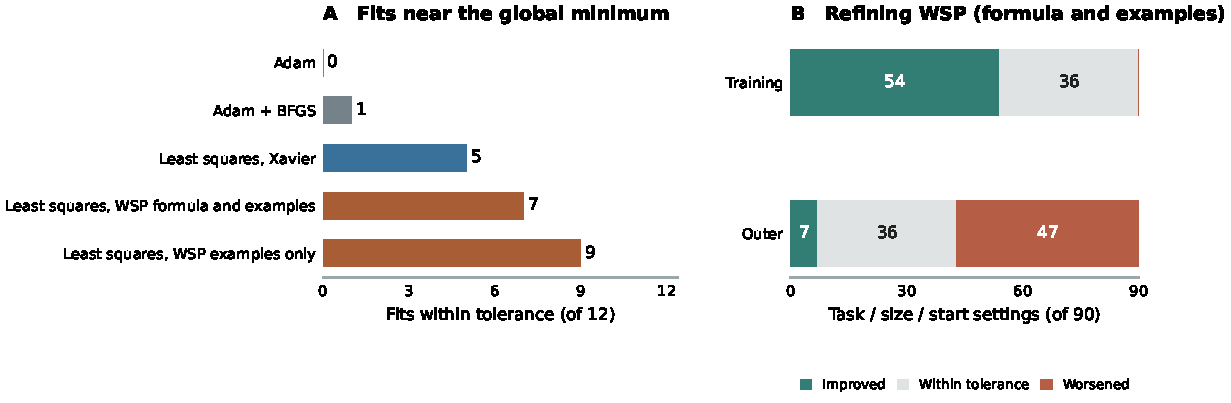
\includegraphics[width=\linewidth]{optimizer.pdf}
\caption{Optimization of the central labels and transfer to the outer shell. Panel a counts fits whose observed loss lies within $10^{-10}$ of the certified real minimum across 12 one-hinge settings. Panel b starts from formula-and-examples WSP and refines each of 90 arrays by least squares. Lower is better. An absolute change of at most $10^{-10}$ is classified as within tolerance. Training uses half the mean squared scaled error, and outer evaluation here uses mean scaled absolute error. Table~\ref{tab:paired} gives raw RMSE in output units.}\label{fig:optim}
\end{figure}

\paragraph{How did conventional recurrent networks fare?}
A hyperbolic-tangent recurrent cell applies $\tanh$ to its updated state. A gated recurrent unit (GRU) uses gates, numbers between zero and one computed from the current input and previous state, to regulate state retention and updating. We trained both on running sums, Fibonacci and triangular recurrences with two variable starting values, and list sorting in which a shared cell first reads a list and then emits its sorted elements. All 102 task, cell, width and initialization settings were fit at two budgets. None of the resulting 204 fits returned a complete exact example on any of the four held-out sets (central, changed magnitude, changed length, or both). A different one-state $\tanh$ cell, with its hidden scale fixed to $2^{-40}$ and two weights learned from ordinary central labels, learned the exact running sum in three of five starts. Each successful start matched all 1,024 outer length-32 streams, with zero RMSE. Appendix~\ref{app:passive-rnn} gives the update equations, unscaled errors and the separate results for the WSP state scaling.
